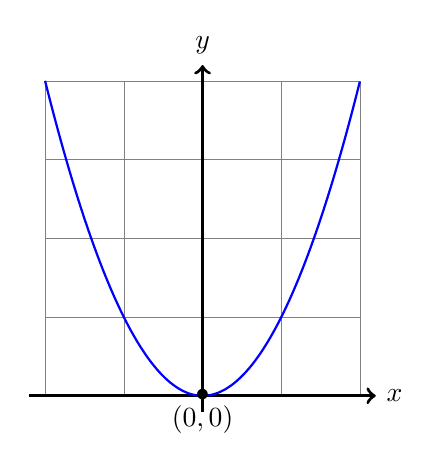
\begin{tikzpicture}
  \draw[very thin,color=gray] (-2,0) grid (2,4);

  \draw[very thick,->] (-2.2,0) -- (2.2,0) node[right] {$x$};
  \draw[very thick,->] (0,-0.2) -- (0,4.2) node[above] {$y$};
  
  \draw [color=blue,thick] plot[smooth,samples=500,domain=-2:2] (\x,{(\x)^2});

  \node at (0,0) {$\bullet$};
  \node [below] at (0,0) {$(0,0)$};
  
  %% \node at (1,-1) {$\bullet$};
  %% \node [above right] at (1,-1) {$(1,-1)$};
\end{tikzpicture}
